\documentclass[11pt]{article}
% Pretty much all of the ams maths packages
\usepackage{amsmath,amsthm,amssymb,amsfonts}
% Allows you to manipulate the page a bit
\usepackage[a4paper]{geometry}
% Pulls the page out a bit - makes it look better (in my opinion)
\usepackage{a4wide}
\usepackage[utf8]{inputenc}
\usepackage[danish,english]{babel}
\usepackage{float}
% Removes paragraph indentation (not needed most of the time now)
\usepackage{parskip}
% Allows inclusion of graphics easily and configurably
\usepackage{graphicx}
% Provides ways to make nice looking tables
\usepackage{booktabs}
% Allows you to rotate tables and figures
\usepackage{rotating}
% Allows shading of table cells
\usepackage{colortbl}
% Define a simple command to use at the start of a table row to make it have a shaded background
\newcommand{\gray}{\rowcolor[gray]{.9}}
\usepackage{textcomp}
% Provides commands to make subfigures (figures with (a), (b) and (c))
\usepackage{subfigure}
% Typesets URLs sensibly - with tt font, clickable in PDFs, and not breaking across lines
\usepackage{url}
% Makes references hyperlinks in PDF output
\usepackage{hyperref}
% Provides ways to include syntax-highlighted source code
\usepackage{listings}
\lstset{frame=single, basicstyle=\ttfamily}
% Provides Harvard-style referencing
\usepackage{natbib}
\bibpunct{(}{)}{;}{a}{,}{,}
% Provides good access to colours
\usepackage{color}
\usepackage{xcolor}
% Simple command I defined to allow me to mark TODO items in red
\newcommand{\todo}[1] {\textbf{\textcolor{red}{#1}}}
% Allows fancy stuff in the page header
\usepackage{fancyhdr}

% Vastly improves the standard formatting of captions
\usepackage[margin=10pt,font=small,labelfont=bf, labelsep=endash]{caption}
% Standard title, author etc.
\title{Dat-F Eksamen Januar 2018}
\author{Christopher Toft Carman - GRP569}
\date{}
% Put text on the left-hand and right-hand side of the header
\begin{document}
\maketitle
\newpage

\section{Introduction} % (fold)
\label{sec:introduction}
Formålet med denne opgave er simulere et simpelt jordskælv ved brug af en forsimplet model. 
Jordskælv sker hvor de tektoniske plader støder sammen og derved udleder en masse energi da der sker en forskydning af pladerne. 
Da det er en kompleks model at beskrive, benytter man sig af forsimplede modeller så som SOC modellen, som bliver brugt i denne opgave.
Soc modellen beskriver at et system med mange frihedsgrader, befinder sig tæt på grænsen til at være stabil, dette medfører altså at små ændringer i systemet kan frigøre energi. 
Formålet her er således at beskrive et simpelt system, og få forståelse for problemet. 

% section introduction (end)

\section{Beskrivelse} % (fold)
\label{sec:beskrivelse}
\subsection{Program Flow} % (fold)
\label{sub:program_flow}
Programmet virker i store træk ligesom `bredte først' algoritmen som er beskrevet på side 6 i opgave beskrivelsen, som kan ses på figur\ref{fig:bredte}. Dog har vi nogle afvigelser, og forskellige måder at opsætte koden på. 
\begin{figure}
  \caption{Her er vist Bredte før algoritmen fra opgave beskrivelsen, hvor forskydelsen breder sig ud som ringe i ens matrice.}
  \label{fig:bredte}
  \centering
    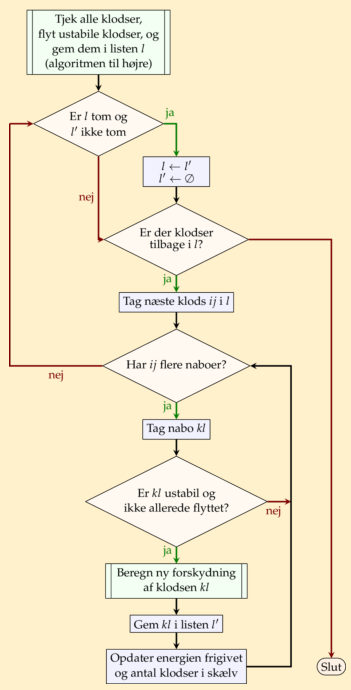
\includegraphics[width=0.5\textwidth]{bredteForst.png}
\end{figure}

Jeg startede med at lave et grid af klodser, eller et mesh af klodser. Her blev der gjort nogle tanker om hvorledes man skal gemme værdierne for hver klods, jeg gjorde mig overvejelser om man skulle bruge objekter til dette. \tabularnewline
Jeg kom fra ideen igen, da object orienterede programmering i MatLab ikke falder mig så let ind imodsætning til andre sprog. Derved bruger jeg structure arrays istedet hvor man får det bedste fra både object orienteret programmering og proceduremæssig programmering. \\
	
Helt overordnet starter jeg med at lave et N x M structure array (struct), og gemmer en masse værdier tilhørende klodserne i. F.eks. bliver klodsernes position, friktions kraft, om de er blevet flyttet osv. gemt. \\

Så tjekker vi igennem alle klodserne og tjekker om de er ustabile eller ej, hvis de er flytter vi dem og noterer dem til en liste.

Der bliver så tjekket igennem alle dem der er flyttet, hvis deres naboer nu er blevet ustabile. Hvis dette altså er tilfældet flytter vi dem og gemmer dem til deres egen liste. 

I det vi er færdige med at tjekke alle naboerne til vores ustabile, kan vores nabo liste så blive til vores ustabile liste, og derved kan processen startes forfra. Dette betyder altså at skælvene vil brede sig ud fra starten som ringe. 

Vi notere så energien for hvert skælv. Selve processen med mit eget flow diagram kan ses på figure 
% subsection program_flow (end)
\subsection{Hvordan Virker det ? } % (fold)
\label{sub:hvordan_virker_det_}
Der blev gjort en masse tanker om hvilken metode der var bedst, jeg valgte blot at bruge 
`'bredte først' algoritmen da den virkede sjov at lave. \\
Her har jeg så en main fil, som er meningen skal køres kaldet pineapple.m, så har jeg nogle andre funktioner som der bliver udnyttet i løbet af programmet. f.eks. tjekKlodser() som tjekker alle klodserne i systemet og fortæller dem om de er ustabile og derefter flytter på den hvor den udnytter funktionen  flytKlods() som tager en klods og flytter den i henhold til den måde der er beskrevet i opgave beskrivelsen. Denne function holder også styr på energien ved den flytning af klods. \\
Derudover har vi funktionerne updateFhor og updateKlods, hvilke begge to ændre den horisontale kraft på klodserne. Den ene berøre dog kun en specifik klods, og den anden berøre alle.


% subsection hvordan_virker_det_ (end)


% section beskrivelse (end)

\section{Opsumering} % (fold)
\label{sec:}
% section  (end)

\end{document}